% =============================================================================
%  microgpt: Beamer presentation
%  Build: latexmk -pdf slides.tex
% =============================================================================
\documentclass[aspectratio=169,11pt]{beamer}
\usepackage[T1]{fontenc}
\usepackage[utf8]{inputenc}
\usepackage[sfdefault]{FiraSans}
\usepackage[scaled=0.9]{inconsolata}
\usetheme[progressbar=frametitle,numbering=fraction,block=fill]{metropolis}
\usepackage{amsmath,bm,mathtools}
\usepackage{booktabs,tabularx,array}
\usepackage{tikz}
\usetikzlibrary{arrows.meta,positioning,fit,backgrounds,calc,shapes.misc}
\usepackage{pgfplots}
\pgfplotsset{compat=1.18}
\usepackage{listings}
\usepackage{xcolor}
\usepackage[backend=biber,style=authoryear-comp,maxcitenames=2,maxbibnames=6,
            giveninits=true,uniquename=false,uniquelist=false,sorting=nyt,dashed=false]{biblatex}
\addbibresource{refs.bib}
\renewcommand*{\bibfont}{\scriptsize}
\usepackage{hyperref}

% ----- colours & code --------------------------------------------------------
\definecolor{accent}{HTML}{B45309}
\definecolor{accent2}{HTML}{1D4ED8}
\definecolor{codebg}{HTML}{F7F7F5}
\definecolor{kw}{HTML}{7C3AED}
\definecolor{str}{HTML}{047857}
\definecolor{cmt}{HTML}{6B7280}
\definecolor{boxbg}{HTML}{FFF7ED}
\definecolor{boxbg2}{HTML}{EFF6FF}
\definecolor{ink}{HTML}{1F2937}
\lstdefinestyle{py}{language=Python,basicstyle=\ttfamily\scriptsize,
  keywordstyle=\color{kw}\bfseries,stringstyle=\color{str},commentstyle=\color{cmt}\itshape,
  showstringspaces=false,columns=fullflexible,keepspaces=true,breaklines=true,
  backgroundcolor=\color{codebg},frame=none,xleftmargin=4pt,xrightmargin=4pt,
  aboveskip=4pt,belowskip=4pt,tabsize=4}
\lstset{style=py}
\newcommand{\code}[1]{\lstinline[basicstyle=\ttfamily\small]|#1|}
\newcommand{\R}{\mathbb{R}}
\newcommand{\softmax}{\operatorname{softmax}}
\newcommand{\rmsnorm}{\operatorname{rmsnorm}}
\newcommand{\relu}{\operatorname{relu}}
\newcommand{\dd}[2]{\frac{\partial #1}{\partial #2}}
\setbeamertemplate{bibliography item}{}
\setbeamerfont{footnote}{size=\tiny}

\title{microgpt}
\subtitle{The complete algorithm of a GPT in 200 lines of Python}
\author{Slides built on Andrej Karpathy's \emph{microgpt} post, 12 Feb 2026}
\date{\today}

\begin{document}
\maketitle

\begin{frame}{Outline}
\small
\begin{columns}[t]
\column{0.5\textwidth}\tableofcontents[hideallsubsections,sections={1-6}]
\column{0.5\textwidth}\tableofcontents[hideallsubsections,sections={7-12}]
\end{columns}
\end{frame}

% =============================================================================
\section{Orientation}
% =============================================================================
\begin{frame}{What microgpt is}
\begin{itemize}
  \item One file, \textbf{200 lines of pure Python}, imports only \texttt{os}, \texttt{math}, \texttt{random}.
  \item Downloads 32{,}033 names, trains a tiny GPT for 1{,}000 steps, prints 20 invented names.
  \item Contains every \emph{algorithmic} ingredient: dataset, tokenizer, autograd, GPT-2-style Transformer, Adam, training loop, inference loop.
  \item Culmination of micrograd $\to$ makemore $\to$ nanoGPT $\to$ llm.c \parencite{karpathy2020micrograd,karpathy2022makemore,karpathy2022nanogpt,karpathy2024llmc}.
\end{itemize}
\begin{block}{Karpathy's claim}
``Everything else is just efficiency. I cannot simplify this any further.'' \parencite{karpathy2026microgpt}
\end{block}
\end{frame}

\begin{frame}{Where to find it}
\begin{itemize}
  \item Blog post: \url{https://karpathy.github.io/2026/02/12/microgpt/}
  \item Gist \texttt{microgpt.py}: \url{https://gist.github.com/karpathy/8627fe009c40f57531cb18360106ce95}
  \item Step-by-step build \texttt{build\_microgpt.py} (revisions \texttt{train0.py} \dots\ \texttt{train5.py}) \parencite{karpathy2026buildmicrogpt}
  \item Colab notebook \parencite{karpathy2026microgptcolab}; web rendering at \url{https://karpathy.ai/microgpt.html}
\end{itemize}
\vfill
\texttt{python microgpt.py} \quad -- nothing to install.
\end{frame}

\begin{frame}{The pipeline}
\centering
\resizebox{0.95\textwidth}{!}{%
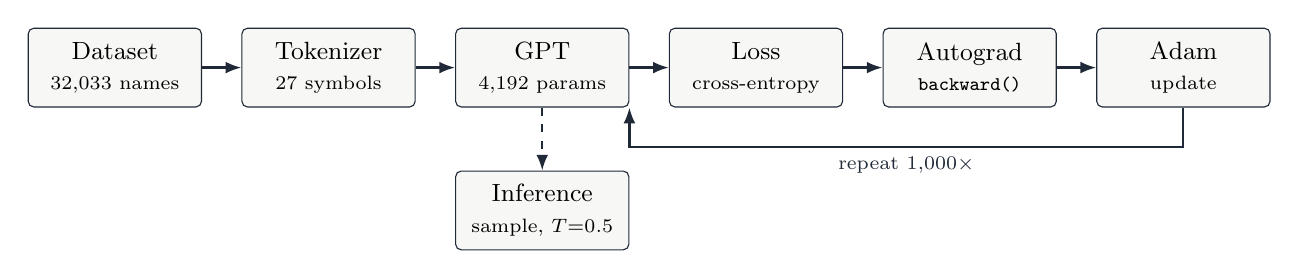
\begin{tikzpicture}[
  node distance=4mm and 5mm,
  box/.style={draw=ink,rounded corners=2pt,fill=codebg,minimum height=10mm,minimum width=22mm,align=center,font=\small},
  arr/.style={-{Latex[length=2mm]},thick,ink}]
\node[box] (data) {Dataset\\ \scriptsize 32{,}033 names};
\node[box,right=of data] (tok) {Tokenizer\\ \scriptsize 27 symbols};
\node[box,right=of tok] (model) {GPT\\ \scriptsize 4{,}192 params};
\node[box,right=of model] (loss) {Loss\\ \scriptsize cross-entropy};
\node[box,right=of loss] (grad) {Autograd\\ \scriptsize \texttt{backward()}};
\node[box,right=of grad] (opt) {Adam\\ \scriptsize update};
\node[box,below=8mm of model] (inf) {Inference\\ \scriptsize sample, $T{=}0.5$};
\draw[arr] (data)--(tok); \draw[arr] (tok)--(model); \draw[arr] (model)--(loss);
\draw[arr] (loss)--(grad); \draw[arr] (grad)--(opt);
\draw[arr] (opt.south) |- ++(0,-5mm) -| node[pos=0.25,below,font=\scriptsize]{repeat $1{,}000\times$} (model.south east);
\draw[arr,dashed] (model.south) -- (inf.north);
\end{tikzpicture}}
\vfill
\small Notation: $V{=}27$ tokens, $d{=}16$ (\code{n_embd}), $H{=}4$ heads, $d_h{=}4$, $L{=}1$ layer, $T_{\max}{=}16$ (\code{block_size}).
\end{frame}

% =============================================================================
\section{Dataset}
% =============================================================================
\begin{frame}[fragile]{Dataset: a list of documents}
\begin{lstlisting}
if not os.path.exists('input.txt'):
    import urllib.request
    urllib.request.urlretrieve(names_url, 'input.txt')  # names.txt from the makemore repo
docs = [line.strip() for line in open('input.txt') if line.strip()]
random.shuffle(docs)
\end{lstlisting}
\begin{columns}
\column{0.45\textwidth}
\texttt{emma, olivia, ava, isabella, sophia, charlotte, mia, amelia, harper, \dots}

32{,}033 names; longest is 15 letters.
\column{0.5\textwidth}
\begin{itemize}
  \item Each name is one \emph{document}.
  \item Production: web pages, books, code, trillions of tokens.
  \item Nothing downstream depends on \emph{what} the documents are.
\end{itemize}
\end{columns}
\end{frame}

\begin{frame}{A conversation is just a document}
\begin{block}{Key idea}
From the model's point of view, a ChatGPT conversation is a single, oddly formatted document. The prompt is a prefix; the reply is a statistical \emph{completion}, one token at a time.
\end{block}
\begin{itemize}
  \item microgpt completing \emph{k-a-r} $\to$ \emph{karai} and ChatGPT completing a prompt into a paragraph are the same operation.
  \item Lineage: Shannon's letter-prediction experiments \parencite{shannon1951prediction}, neural LMs \parencite{bengio2003neural}, character-level RNNs \parencite{sutskever2011generating,graves2013generating,karpathy2015rnn}.
\end{itemize}
\end{frame}

% =============================================================================
\section{Tokenizer}
% =============================================================================
\begin{frame}[fragile]{Tokenizer: characters as discrete symbols}
\begin{lstlisting}
uchars = sorted(set(''.join(docs))) # unique characters -> ids 0..n-1
BOS = len(uchars)                   # special Beginning of Sequence token
vocab_size = len(uchars) + 1        # 26 letters + BOS = 27
\end{lstlisting}
\begin{itemize}
  \item \texttt{a}$\mapsto 0$, \dots, \texttt{z}$\mapsto 25$, \texttt{BOS}$\mapsto 26$. Encode: \code{uchars.index(ch)}; decode: \code{uchars[id]}.
  \item Ids have \textbf{no arithmetic meaning}: ``they might as well be different emoji''.
  \item \texttt{BOS} wraps every document: \texttt{[BOS, e, m, m, a, BOS]} -- it starts a name and ends one.
\end{itemize}
\end{frame}

\begin{frame}{Production tokenizers: byte-pair encoding}
\begin{itemize}
  \item BPE: start from bytes, repeatedly merge the most frequent adjacent pair \parencite{gage1994bpe,sennrich2016bpe}.
  \item GPT-2: $\sim$50K tokens; GPT-4 / tiktoken: $\sim$100K \parencite{radford2019gpt2,openai2022tiktoken}.
  \item Common words become one token; rare words split into pieces $\Rightarrow$ more content per position.
  \item SentencePiece is the other common implementation \parencite{kudo2018sentencepiece}.
  \item Next step after this course: Karpathy's tokenizer lecture \parencite{karpathy2024tokenizervideo}.
\end{itemize}
\end{frame}

% =============================================================================
\section{Autograd}
% =============================================================================
\begin{frame}{Why gradients}
\begin{itemize}
  \item Training adjusts each parameter $\theta$ to lower the loss $\mathcal L$: we need $\partial\mathcal L/\partial\theta$.
  \item ``If I nudge this number up a little, does the loss go up or down, and by how much?''
  \item Thousands of inputs, \textbf{one} scalar output $\Rightarrow$ reverse-mode autodiff (backpropagation): one backward sweep gives all gradients.
  \item History: \textcite{linnainmaa1976taylor}, \textcite{rumelhart1986learning}; survey: \textcite{baydin2018autodiff}.
\end{itemize}
\end{frame}

\begin{frame}[fragile]{The \texttt{Value} class: forward}
\begin{lstlisting}
class Value:
    __slots__ = ('data', 'grad', '_children', '_local_grads')
    def __init__(self, data, children=(), local_grads=()):
        self.data = data; self.grad = 0
        self._children = children; self._local_grads = local_grads
    def __add__(self, other):
        other = other if isinstance(other, Value) else Value(other)
        return Value(self.data + other.data, (self, other), (1, 1))
    def __mul__(self, other):
        other = other if isinstance(other, Value) else Value(other)
        return Value(self.data * other.data, (self, other), (other.data, self.data))
    def __pow__(self, other): return Value(self.data**other, (self,), (other * self.data**(other-1),))
    def log(self):  return Value(math.log(self.data), (self,), (1/self.data,))
    def exp(self):  return Value(math.exp(self.data), (self,), (math.exp(self.data),))
    def relu(self): return Value(max(0, self.data), (self,), (float(self.data > 0),))
\end{lstlisting}
\vspace{-2pt}{\small Each operation returns a new node remembering its inputs and its \emph{local} derivative.}
\end{frame}

\begin{frame}{The six lego blocks}
\centering
\begin{tabular}{@{}lll@{}}
\toprule
Operation & Forward & Local gradients \\
\midrule
\texttt{a + b} & $a+b$ & $1,\ 1$ \\
\texttt{a * b} & $ab$ & $b,\ a$ \\
\texttt{a ** n} & $a^n$ & $n a^{n-1}$ \\
\texttt{a.log()} & $\ln a$ & $1/a$ \\
\texttt{a.exp()} & $e^a$ & $e^a$ \\
\texttt{a.relu()} & $\max(0,a)$ & $\mathbf 1[a>0]$ \\
\bottomrule
\end{tabular}
\vfill
Subtraction, division and negation are derived: \texttt{a - b = a + (-1)*b}, \texttt{a / b = a * b**-1}.
\end{frame}

\begin{frame}[fragile]{The \texttt{Value} class: backward}
\begin{columns}
\column{0.5\textwidth}
\begin{lstlisting}
def backward(self):
    topo, visited = [], set()
    def build_topo(v):
        if v not in visited:
            visited.add(v)
            for child in v._children:
                build_topo(child)
            topo.append(v)
    build_topo(self)
    self.grad = 1
    for v in reversed(topo):
        for child, lg in zip(v._children, v._local_grads):
            child.grad += lg * v.grad
\end{lstlisting}
\column{0.48\textwidth}
\begin{enumerate}
  \item \textbf{Topological sort} by DFS: children before parents.
  \item \textbf{Seed} $\partial\mathcal L/\partial\mathcal L = 1$.
  \item \textbf{Chain rule}, root to leaves:
  \[\dd{\mathcal L}{c} \mathrel{+}= \dd{v}{c}\cdot\dd{\mathcal L}{v}\]
\end{enumerate}
The \texttt{+=} sums contributions when a node feeds several parents (multivariable chain rule).
\end{columns}
\end{frame}

\begin{frame}[fragile]{Worked example: $L = ab + a$}
\begin{columns}
\column{0.42\textwidth}
\begin{lstlisting}
a = Value(2.0); b = Value(3.0)
c = a * b       # 6.0
L = c + a       # 8.0
L.backward()
print(a.grad)   # 4.0
print(b.grad)   # 2.0
\end{lstlisting}
PyTorch gives \texttt{tensor(4.)}, \texttt{tensor(2.)}: same algorithm, on tensors.
\column{0.56\textwidth}
\centering
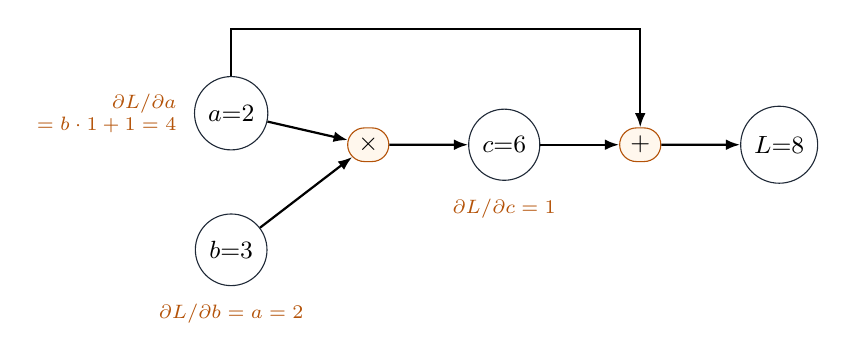
\begin{tikzpicture}[
  node distance=8mm and 10mm,
  v/.style={draw=ink,circle,minimum size=8mm,font=\small,fill=white},
  op/.style={draw=accent,rounded rectangle,fill=boxbg,font=\small,inner sep=3pt},
  arr/.style={-{Latex[length=1.8mm]},thick},
  g/.style={font=\scriptsize,accent}]
\node[v] (a) {$a{=}2$};
\node[v,below=of a] (b) {$b{=}3$};
\node[op,right=of a,yshift=-4mm] (mul) {$\times$};
\node[v,right=of mul] (c) {$c{=}6$};
\node[op,right=of c] (add) {$+$};
\node[v,right=of add] (L) {$L{=}8$};
\draw[arr] (a)--(mul); \draw[arr] (b)--(mul); \draw[arr] (mul)--(c);
\draw[arr] (c)--(add); \draw[arr] (add)--(L);
\draw[arr] (a.north) -- ++(0,6mm) -| (add.north);
\node[g,below=1mm of b] {$\partial L/\partial b = a = 2$};
\node[g,below=1mm of c] {$\partial L/\partial c = 1$};
\node[g,left=1mm of a,align=right] {$\partial L/\partial a$\\$= b\cdot 1 + 1 = 4$};
\end{tikzpicture}
\end{columns}
\vfill
Meaning: raising $a$ by $0.001$ raises $L$ by about $0.004$. Sign = direction, magnitude = steepness.
\end{frame}

\begin{frame}{Scalars vs.\ tensors}
\begin{itemize}
  \item microgpt: one graph node per scalar operation. One training step on ``christopher'' builds $\approx 10^5$ nodes.
  \item PyTorch \parencite{paszke2017autodiff,paszke2019pytorch}: one node per \emph{tensor} operation; a backward node can be a fused GPU kernel.
  \item ``Algorithmically identical, significantly smaller and simpler, but of course a lot less efficient.''
\end{itemize}
\vfill
\centering
\begin{tabular}{@{}lrrrr@{}}
\toprule
Document & $n$ & \texttt{Value} nodes & forward (s) & backward (s)\\
\midrule
emma & 5 & 39{,}703 & 0.055 & 0.038 \\
isabella & 9 & 73{,}263 & 0.161 & 0.069 \\
christopher & 12 & 99{,}483 & 0.251 & 0.099 \\
\bottomrule
\end{tabular}
\end{frame}

% =============================================================================
\section{Parameters}
% =============================================================================
\begin{frame}[fragile]{Parameters: the knowledge of the model}
\begin{lstlisting}
n_layer, n_embd, block_size, n_head = 1, 16, 16, 4
head_dim = n_embd // n_head
matrix = lambda nout, nin, std=0.08: [[Value(random.gauss(0, std)) for _ in range(nin)] for _ in range(nout)]
state_dict = {'wte': matrix(vocab_size, n_embd), 'wpe': matrix(block_size, n_embd), 'lm_head': matrix(vocab_size, n_embd)}
for i in range(n_layer):
    state_dict[f'layer{i}.attn_wq'] = matrix(n_embd, n_embd)
    state_dict[f'layer{i}.attn_wk'] = matrix(n_embd, n_embd)
    state_dict[f'layer{i}.attn_wv'] = matrix(n_embd, n_embd)
    state_dict[f'layer{i}.attn_wo'] = matrix(n_embd, n_embd)
    state_dict[f'layer{i}.mlp_fc1'] = matrix(4 * n_embd, n_embd)
    state_dict[f'layer{i}.mlp_fc2'] = matrix(n_embd, 4 * n_embd)
params = [p for mat in state_dict.values() for row in mat for p in row]
\end{lstlisting}
Small Gaussian init ($\sigma = 0.08$); named matrices in a \texttt{state\_dict}; flat list \texttt{params} for the optimizer.
\end{frame}

\begin{frame}{Counting to 4{,}192}
\centering
\begin{tabular}{@{}llrr@{}}
\toprule
Name & Shape & & Count \\
\midrule
\texttt{wte} & $V\times d$ & $27\times 16$ & 432 \\
\texttt{wpe} & $T_{\max}\times d$ & $16\times 16$ & 256 \\
\texttt{lm\_head} & $V\times d$ & $27\times 16$ & 432 \\
\texttt{attn\_wq/wk/wv/wo} & $4\,(d\times d)$ & $4\times 256$ & 1{,}024 \\
\texttt{mlp\_fc1} & $4d\times d$ & $64\times 16$ & 1{,}024 \\
\texttt{mlp\_fc2} & $d\times 4d$ & $16\times 64$ & 1{,}024 \\
\midrule
Total & & & \textbf{4{,}192} \\
\bottomrule
\end{tabular}
\vfill
Per layer: $12d^2$ (attention $4d^2$ + MLP $8d^2$). GPT-2: 1.5B; GPT-3: 175B \parencite{radford2019gpt2,brown2020gpt3}. No biases, no weight tying \parencite{press2017weighttying}, init scale cf.\ \textcite{glorot2010init}.
\end{frame}

% =============================================================================
\section{Architecture}
% =============================================================================
\begin{frame}[fragile]{Three helpers}
\begin{lstlisting}
def linear(x, w):            # matrix-vector product: one dot product per row of w
    return [sum(wi * xi for wi, xi in zip(wo, x)) for wo in w]

def softmax(logits):         # scores -> probabilities; subtract max for stability
    max_val = max(val.data for val in logits)
    exps = [(val - max_val).exp() for val in logits]
    total = sum(exps)
    return [e / total for e in exps]

def rmsnorm(x):              # rescale to unit root-mean-square (no learned gain)
    ms = sum(xi * xi for xi in x) / len(x)
    scale = (ms + 1e-5) ** -0.5
    return [xi * scale for xi in x]
\end{lstlisting}
\[
\softmax(z)_i = \frac{e^{z_i-m}}{\sum_j e^{z_j-m}},\qquad
\rmsnorm(x) = \frac{x}{\sqrt{\frac1d\sum_i x_i^2+\varepsilon}}\quad\text{\parencite{zhang2019rmsnorm}}
\]
\end{frame}

\begin{frame}[fragile]{The model function (1/3): embeddings and attention}
\begin{lstlisting}[basicstyle=\ttfamily\tiny]
def gpt(token_id, pos_id, keys, values):
    tok_emb = state_dict['wte'][token_id]; pos_emb = state_dict['wpe'][pos_id]
    x = [t + p for t, p in zip(tok_emb, pos_emb)]
    x = rmsnorm(x) # note: not redundant due to backward pass via the residual connection
    for li in range(n_layer):
        # 1) Multi-head Attention block
        x_residual = x
        x = rmsnorm(x)
        q = linear(x, state_dict[f'layer{li}.attn_wq'])
        k = linear(x, state_dict[f'layer{li}.attn_wk'])
        v = linear(x, state_dict[f'layer{li}.attn_wv'])
        keys[li].append(k); values[li].append(v)
\end{lstlisting}
Embeddings, the first \texttt{rmsnorm}, the pre-norm, the $q,k,v$ projections, and the cache append.
\end{frame}

\begin{frame}[fragile]{The model function (2/3): the head loop}
\begin{lstlisting}[basicstyle=\ttfamily\tiny]
        x_attn = []
        for h in range(n_head):
            hs = h * head_dim
            q_h = q[hs:hs+head_dim]
            k_h = [ki[hs:hs+head_dim] for ki in keys[li]]
            v_h = [vi[hs:hs+head_dim] for vi in values[li]]
            attn_logits = [sum(q_h[j] * k_h[t][j] for j in range(head_dim)) / head_dim**0.5 for t in range(len(k_h))]
            attn_weights = softmax(attn_logits)
            head_out = [sum(attn_weights[t] * v_h[t][j] for t in range(len(v_h))) for j in range(head_dim)]
            x_attn.extend(head_out)
        x = linear(x_attn, state_dict[f'layer{li}.attn_wo'])
        x = [a + b for a, b in zip(x, x_residual)]
\end{lstlisting}
Per head: slice $q,k,v$; scaled dot products with every cached key; softmax; weighted sum of cached values. Concatenate heads, project with $W_o$, add the residual.
GPT-2 \parencite{radford2019gpt2} with: LayerNorm $\to$ RMSNorm, no biases, GeLU $\to$ ReLU.
\end{frame}

\begin{frame}[fragile]{The model function (3/3): MLP and output}
\begin{lstlisting}[basicstyle=\ttfamily\scriptsize]
        # 2) MLP block
        x_residual = x
        x = rmsnorm(x)
        x = linear(x, state_dict[f'layer{li}.mlp_fc1'])
        x = [xi.relu() for xi in x]
        x = linear(x, state_dict[f'layer{li}.mlp_fc2'])
        x = [a + b for a, b in zip(x, x_residual)]

    logits = linear(x, state_dict['lm_head'])
    return logits
\end{lstlisting}
\begin{itemize}
  \item Each block: $x \leftarrow x + f(\rmsnorm(x))$, the \emph{pre-norm} residual pattern of GPT-2.
  \item MLP: $W_2\,\relu(W_1 x)$ with $W_1\in\R^{64\times16}$, $W_2\in\R^{16\times64}$; fully local to one position.
  \item \texttt{lm\_head} maps the final $x\in\R^{16}$ to 27 logits. Softmax is applied by the caller.
\end{itemize}
\end{frame}

\begin{frame}{The architecture, one token at a time}
\centering
\resizebox{\textwidth}{!}{%
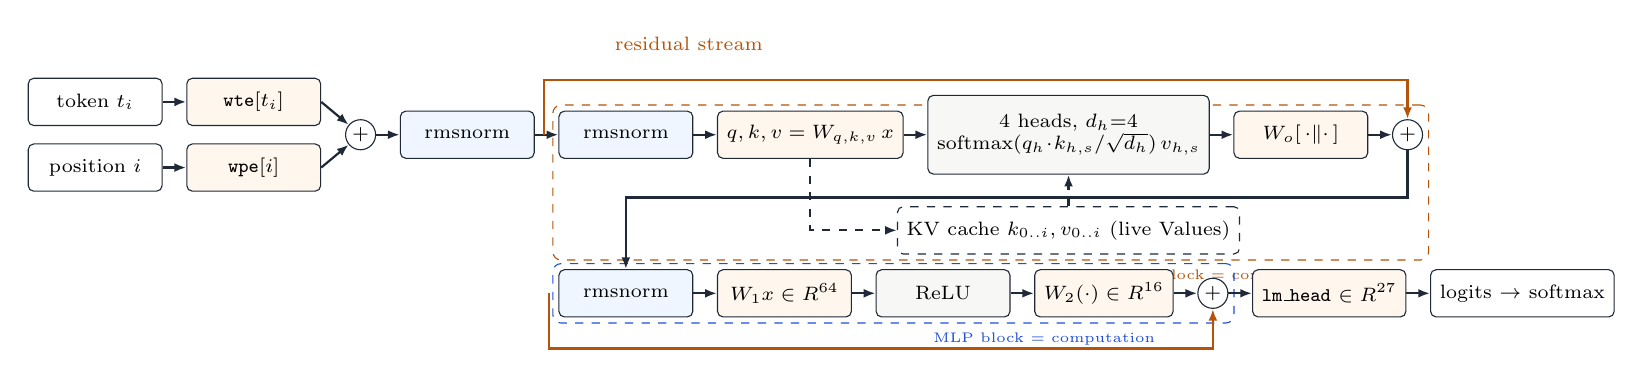
\begin{tikzpicture}[
  font=\scriptsize,
  node distance=2.2mm and 3mm,
  blk/.style={draw=ink,rounded corners=2pt,fill=codebg,minimum width=17mm,minimum height=6mm,align=center},
  prm/.style={blk,fill=boxbg},
  nrm/.style={blk,fill=boxbg2},
  add/.style={draw=ink,circle,inner sep=1pt,fill=white,font=\scriptsize},
  arr/.style={-{Latex[length=1.5mm]},thick,ink}]
% row 1: embeddings + attention
\node[blk,fill=white] (tok) {token $t_i$};
\node[blk,fill=white,below=of tok] (pos) {position $i$};
\node[prm,right=of tok] (wte) {\texttt{wte}$[t_i]$};
\node[prm,right=of pos] (wpe) {\texttt{wpe}$[i]$};
\node[add] (add0) at ($(wte.east)!0.5!(wpe.east)+(5mm,0)$) {$+$};
\node[nrm,right=of add0] (n0) {rmsnorm};
\node[nrm,right=of n0] (n1) {rmsnorm};
\node[prm,right=of n1] (qkv) {$q,k,v = W_{q,k,v}\,x$};
\node[blk,right=of qkv,minimum width=26mm,minimum height=10mm] (attn) {4 heads, $d_h{=}4$\\ softmax$(q_h\!\cdot\!k_{h,s}/\sqrt{d_h})\,v_{h,s}$};
\node[prm,right=of attn] (wo) {$W_o[\,\cdot\|\cdot\,]$};
\node[add,right=of wo] (add1) {$+$};
\node[blk,fill=white,dashed,below=4mm of attn,minimum width=26mm] (kv) {KV cache $k_{0..i},v_{0..i}$ (live Values)};
% row 2: MLP + head
\node[nrm,below=14mm of n1] (n2) {rmsnorm};
\node[prm,right=of n2] (fc1) {$W_1x\in\R^{64}$};
\node[blk,right=of fc1] (relu) {ReLU};
\node[prm,right=of relu] (fc2) {$W_2(\cdot)\in\R^{16}$};
\node[add,right=of fc2] (add2) {$+$};
\node[prm,right=of add2] (lm) {\texttt{lm\_head} $\in\R^{27}$};
\node[blk,fill=white,right=of lm] (out) {logits $\to$ softmax};
% arrows
\draw[arr] (tok)--(wte); \draw[arr] (pos)--(wpe);
\draw[arr] (wte.east)--(add0); \draw[arr] (wpe.east)--(add0);
\draw[arr] (add0)--(n0); \draw[arr] (n0)--(n1); \draw[arr] (n1)--(qkv); \draw[arr] (qkv)--(attn); \draw[arr] (attn)--(wo); \draw[arr] (wo)--(add1);
\draw[arr,dashed] (qkv.south) |- (kv.west); \draw[arr,dashed] (kv.north) -- (attn.south);
\draw[arr] (add1.south) |- ++(-3mm,-6mm) -| ($(n2.north)+(0,3mm)$) -- (n2.north);
\draw[arr] (n2)--(fc1); \draw[arr] (fc1)--(relu); \draw[arr] (relu)--(fc2); \draw[arr] (fc2)--(add2); \draw[arr] (add2)--(lm); \draw[arr] (lm)--(out);
% residuals
\draw[arr,accent] ($(n0.east)+(1.2mm,0)$) -- ++(0,7mm) -| (add1.north);
\draw[arr,accent] ($(n2.west)+(-1.2mm,0)$) -- ++(0,-7mm) -| (add2.south);
\node[accent,font=\scriptsize] at ($(n1.north)+(8mm,8.5mm)$) {residual stream};
\begin{scope}[on background layer]
\node[draw=accent,dashed,rounded corners=3pt,fit=(n1)(add1)(kv),inner sep=2pt,label={[accent,font=\tiny]below right:attention block = communication}] {};
\node[draw=accent2,dashed,rounded corners=3pt,fit=(n2)(add2),inner sep=2pt,label={[accent2,font=\tiny]below right:MLP block = computation}] {};
\end{scope}
\end{tikzpicture}}

\vspace{4pt}{\small Orange = parameters, blue = parameter-free normalisation, orange arrows = residual connections. For $L>1$ the two blocks repeat.}
\end{frame}

\begin{frame}{Embeddings}
\[
x^{(0)}_i = \rmsnorm\big(\mathrm{wte}[t_i] + \mathrm{wpe}[i]\big)\in\R^{16}
\]
\begin{itemize}
  \item A network cannot use the symbol ``5''; it looks up a learned vector per token and per position and adds them: \emph{what} + \emph{where}.
  \item Attention is a weighted sum over cached positions, so \texttt{wpe} is the \emph{only} source of order information.
  \item Original Transformer: fixed sinusoids \parencite{vaswani2017attention}; GPT-1/2: learned table; modern: RoPE, relative rotations of $q,k$ \parencite{su2021rope}.
  \item The first \texttt{rmsnorm} fixes the scale at which the residual stream starts; pre-norm inside blocks only touches the branch input.
\end{itemize}
\end{frame}

\begin{frame}{Attention}
\small\vspace{-4pt}
\begin{columns}
\column{0.55\textwidth}
\begin{align*}
q &= W_q x,\quad k = W_k x,\quad v = W_v x \\
a_{h,s} &= \frac{q[S_h]\cdot k_s[S_h]}{\sqrt{d_h}},\qquad s\le i\\
\alpha_h &= \softmax(a_{h,0},\dots,a_{h,i})\\
\mathrm{head}_h &= \textstyle\sum_{s\le i}\alpha_{h,s}\,v_s[S_h]\\
\text{out} &= W_o\,[\mathrm{head}_1\|\cdots\|\mathrm{head}_4]
\end{align*}
\column{0.45\textwidth}
\begin{itemize}
  \item Query ``what am I looking for?'', key ``what do I contain?'', value ``what do I offer?''
  \item $k, v$ appended to the cache each step.
  \item $1/\sqrt{d_h}$ keeps logits at unit variance \parencite{vaswani2017attention}.
  \item 4 heads $\times$ width 4 cost the same as 1 head $\times$ 16; they buy \emph{diversity}.
  \item \textbf{No causal mask needed}: the cache holds only $s\le i$.
\end{itemize}
\end{columns}
\end{frame}

\begin{frame}{Attention is communication; MLP is computation}
\begin{itemize}
  \item The attention block is the \textbf{only} place where position $i$ reads from positions $0..i{-}1$.
  \item MLP: $W_2\,\relu(W_1 x)$, project up $4\times$, nonlinearity, project down. Fully local to one position: ``where the model does most of its thinking''.
  \item GPT-2 used GELU \parencite{hendrycks2016gelu}; modern models use gated SwiGLU \parencite{shazeer2020glu,touvron2023llama} or squared ReLU \parencite{so2021primer}.
  \item Residuals $x \leftarrow x + f(\rmsnorm(x))$ let gradients flow straight through \parencite{he2016resnet}; pre-norm stabilises training \parencite{xiong2020prelayernorm}.
  \item The ``residual stream'' view: blocks read from and write to a shared vector \parencite{elhage2021mathematical}.
\end{itemize}
\end{frame}

\begin{frame}{The KV cache, even during training}
\begin{itemize}
  \item Usually associated with inference; Karpathy: it is ``conceptually always there''.
  \item Vectorised training hides it inside one big attention matmul. microgpt processes one token at a time, so the cache is explicit.
  \item Here cached $k,v$ are \textbf{live} \texttt{Value} nodes: loss at position 7 backpropagates into the parameters that produced $k_2, v_2$.
  \item Cache size $2\,L\,T\,d$ per sequence motivates MQA/GQA \parencite{shazeer2019mqa,ainslie2023gqa} and paged caches in vLLM \parencite{kwon2023vllm}; accounting in \textcite{pope2022efficiently}.
\end{itemize}
\vfill
Cost per token $\approx 12d^2 + Vd + O(i\,d)$ multiply--adds $\approx 2\times$(non-embedding params): the $2N$ / $6N$ rule of \textcite{kaplan2020scaling} already holds.
\end{frame}

% =============================================================================
\section{Training loop}
% =============================================================================
\begin{frame}[fragile]{Training loop: pick a document, forward, loss, backward, update}
\vspace{-4pt}
\begin{lstlisting}[basicstyle=\ttfamily\tiny]
learning_rate, beta1, beta2, eps_adam = 0.01, 0.85, 0.99, 1e-8
m = [0.0] * len(params); v = [0.0] * len(params); num_steps = 1000
for step in range(num_steps):
    doc = docs[step % len(docs)]
    tokens = [BOS] + [uchars.index(ch) for ch in doc] + [BOS]
    n = min(block_size, len(tokens) - 1)
    keys, values = [[] for _ in range(n_layer)], [[] for _ in range(n_layer)]
    losses = []
    for pos_id in range(n):
        token_id, target_id = tokens[pos_id], tokens[pos_id + 1]
        logits = gpt(token_id, pos_id, keys, values)
        probs = softmax(logits)
        loss_t = -probs[target_id].log()
        losses.append(loss_t)
    loss = (1 / n) * sum(losses)   # May yours be low.
    loss.backward()
    lr_t = learning_rate * (1 - step / num_steps)   # linear decay
    for i, p in enumerate(params):
        m[i] = beta1 * m[i] + (1 - beta1) * p.grad
        v[i] = beta2 * v[i] + (1 - beta2) * p.grad ** 2
        m_hat = m[i] / (1 - beta1 ** (step + 1)); v_hat = v[i] / (1 - beta2 ** (step + 1))
        p.data -= lr_t * m_hat / (v_hat ** 0.5 + eps_adam)
        p.grad = 0
\end{lstlisting}
\end{frame}

\begin{frame}{Next-token prediction and cross-entropy}
``emma'' $\to$ \texttt{[BOS, e, m, m, a, BOS]}; position $i$ sees $t_{\le i}$, predicts $t_{i+1}$; $n=5$ predictions.
\[
\ell_i = -\log p(t_{i+1}\mid t_{\le i}),\qquad \mathcal L = \frac1n\sum_{i=0}^{n-1}\ell_i
\]
\begin{columns}
\column{0.5\textwidth}
\textbf{Three views of $-\log p$}
\begin{itemize}
  \item Surprise / surprisal \parencite{shannon1948mathematical}
  \item Maximum likelihood of the corpus
  \item Cross-entropy = entropy + KL \parencite{goodfellow2016deep}
\end{itemize}
\column{0.5\textwidth}
\textbf{Reference values}
\begin{itemize}
  \item Uniform guess: $\ln 27 \approx 3.30$
  \item First step: $3.37$; after 1{,}000 steps: $\approx 2.3$
  \item Perplexity $e^{\mathcal L}$: $27 \to \approx 10$
  \item Bits/char $\mathcal L/\ln 2$: $4.75 \to \approx 3.4$
\end{itemize}
\end{columns}
\vfill
Bonus identity (derived automatically by autograd): $\partial\ell/\partial z_k = p_k - y_k$.
\end{frame}

\begin{frame}{The loss curve (our run, seed 42)}
\centering
\begin{tikzpicture}
\begin{axis}[width=0.92\textwidth,height=0.62\textheight,
  xlabel={training step},ylabel={loss (nats/token)},
  xmin=0,xmax=1000,ymin=1.4,ymax=3.8,grid=major,grid style={gray!30},
  legend pos=south west,legend style={font=\scriptsize,draw=none,fill=white,fill opacity=0.8},
  tick label style={font=\scriptsize},label style={font=\small}]
\addplot[gray!70,only marks,mark=*,mark size=0.5pt,opacity=0.7] table[col sep=comma,x=step,y=loss]{loss.csv};
\addlegendentry{per-document loss}
\addplot[accent,very thick] table[col sep=comma,x=step,y=avg]{loss.csv};
\addlegendentry{trailing 50-step mean}
\addplot[accent2,dashed,thick,domain=0:1000] {ln(27)};
\addlegendentry{$\ln 27$ (uniform)}
\end{axis}
\end{tikzpicture}

\small Batch size one $\Rightarrow$ noisy dots. Only 1{,}000 of 32{,}033 names seen: every step is on fresh data, so this is effectively a held-out loss.
\end{frame}

\begin{frame}{Adam}
\begin{align*}
m_t &= \beta_1 m_{t-1} + (1-\beta_1)g_t, & \hat m_t &= m_t/(1-\beta_1^{\,t}) \\
v_t &= \beta_2 v_{t-1} + (1-\beta_2)g_t^2, & \hat v_t &= v_t/(1-\beta_2^{\,t}) \\
\theta_t &= \theta_{t-1} - \eta_t\,\hat m_t/(\sqrt{\hat v_t}+\epsilon)
\end{align*}
\begin{itemize}
\small
  \item $m$: momentum \parencite{polyak1964momentum}; $v$: per-parameter step size (RMSProp, \citeauthor{tieleman2012rmsprop} \citeyear{tieleman2012rmsprop}); $\hat m,\hat v$: bias corrections \parencite{kingma2015adam}.
  \item microgpt: $\beta_1{=}0.85$, $\beta_2{=}0.99$ (defaults $0.9$, $0.999$); $\eta_t = 0.01\,(1-t/1000)$.
  \item At scale: AdamW + warmup + cosine \parencite{loshchilov2019adamw,loshchilov2017sgdr}. Reset \texttt{.grad = 0} after each step.
\end{itemize}
\end{frame}

% =============================================================================
\section{Inference}
% =============================================================================
\begin{frame}[fragile]{Inference: sampling}
\begin{lstlisting}
temperature = 0.5
for sample_idx in range(20):
    keys, values = [[] for _ in range(n_layer)], [[] for _ in range(n_layer)]
    token_id = BOS
    sample = []
    for pos_id in range(block_size):
        logits = gpt(token_id, pos_id, keys, values)
        probs = softmax([l / temperature for l in logits])
        token_id = random.choices(range(vocab_size), weights=[p.data for p in probs])[0]
        if token_id == BOS:
            break
        sample.append(uchars[token_id])
    print(f"sample {sample_idx+1:2d}: {''.join(sample)}")
\end{lstlisting}
Start from \texttt{BOS}, sample a token, feed it back, stop at \texttt{BOS} or $T_{\max}$: autoregressive (ancestral) sampling.
\end{frame}

\begin{frame}{Temperature}
\small\vspace{-8pt}
\[
p^{(T)}_k = \frac{e^{z_k/T}}{\sum_j e^{z_j/T}}
\]
\begin{columns}
\column{0.5\textwidth}
\begin{itemize}
  \item $T=1$: the learned distribution.
  \item $T<1$: sharper, conservative ($0.5$ here).
  \item $T\to 0$: greedy decoding (arg-max).
  \item $T>1$: flatter, more diverse, less coherent.
\end{itemize}
\column{0.5\textwidth}
\begin{itemize}
  \item Origin: Boltzmann distribution \parencite{ackley1985boltzmann}; see also \textcite{hinton2015distilling}.
  \item Companions: top-$k$ \parencite{fan2018hierarchical}, nucleus sampling \parencite{holtzman2020nucleus}.
\end{itemize}
\end{columns}
\vspace{4pt}
{\small\textbf{Samples (seed 42):} kamon, ann, karai, jaire, vialan, karia, yeran, anna, areli, kaina, konna, keylen, liole, alerin, earan, lenne, kana, lara, alela, anton. Plausible, mostly \emph{not} in the training set: ``hallucination''.}
\end{frame}

% =============================================================================
\section{Run it and build it}
% =============================================================================
\begin{frame}[fragile]{Run it}
\begin{lstlisting}[language=bash]
python microgpt.py
\end{lstlisting}
\begin{lstlisting}[language={}]
num docs: 32033
vocab size: 27
num params: 4192
step    1 / 1000 | loss 3.3660
...
step 1000 / 1000 | loss 2.6497
--- inference (new, hallucinated names) ---
sample  1: kamon
\end{lstlisting}
\begin{itemize}
  \item Karpathy: about 1 minute on his MacBook. Our laptop: 3 min 24 s in CPython.
  \item Knobs: \texttt{num\_steps}, \texttt{n\_embd}, \texttt{n\_layer}, \texttt{n\_head}, \texttt{temperature}, the dataset file.
\end{itemize}
\end{frame}

\begin{frame}{Progression: layers of the onion}
\centering
\begin{tabular}{@{}ll@{}}
\toprule
File & What it adds \\
\midrule
\texttt{train0.py} & Bigram count table: no neural net, no gradients \\
\texttt{train1.py} & MLP + manual gradients (numerical \& analytic) + SGD \\
\texttt{train2.py} & Autograd (\texttt{Value} class) replaces manual gradients \\
\texttt{train3.py} & Position embeddings + single-head attention + rmsnorm + residuals \\
\texttt{train4.py} & Multi-head attention + layer loop: full GPT \\
\texttt{train5.py} & Adam optimizer: this is \texttt{train.py} \\
\bottomrule
\end{tabular}
\vfill
Revisions of \texttt{build\_microgpt.py} \parencite{karpathy2026buildmicrogpt}. Mirrors history: $n$-grams $\to$ neural LMs $\to$ backprop $\to$ attention $\to$ adaptive optimizers.
\end{frame}

% =============================================================================
\section{From microgpt to production}
% =============================================================================
\begin{frame}{What changes at scale (nothing in the algorithm)}
\scriptsize
\begin{tabularx}{\textwidth}{@{}lXX@{}}
\toprule
& microgpt & Production \\
\midrule
Data & 32K names & Trillions of tokens; dedup, filtering, mixing \\
Tokenizer & 27 chars & Byte-level BPE, $\sim$100K tokens \\
Autograd & scalar \texttt{Value} & Tensors on GPUs; fused kernels (FlashAttention) \\
Architecture & 4{,}192 params, $L{=}1$ & $10^{11+}$ params, $L{>}100$; RoPE, GQA, gated MLP, MoE \\
Training & 1 doc/step & Millions of tokens/step, mixed precision, months on thousands of GPUs \\
Optimisation & Adam, linear decay & Tuned AdamW, warmup, scaling laws \\
Post-training & none & SFT then RL \\
Inference & 1 sample at a time & Batching, paged KV, speculative decoding, quantisation \\
\bottomrule
\end{tabularx}
\end{frame}

\begin{frame}{Data, tokenizer, hardware}
\begin{itemize}
  \item \textbf{Data}: web, books, code; deduplication measurably helps \parencite{lee2022dedup}; curated corpora \parencite{raffel2020t5,gao2020pile,penedo2024fineweb}.
  \item \textbf{Tokenizer}: BPE gives $\sim$4 characters per token in English, multiplying effective context.
  \item \textbf{Autograd}: same maths over tensors \parencite{paszke2019pytorch}; FlashAttention tiles attention through on-chip memory without materialising the $T\times T$ matrix \parencite{dao2022flashattention,dao2024flashattention2}.
\end{itemize}
\end{frame}

\begin{frame}{Architecture and training at scale}
\begin{itemize}
  \item Residual stream of attention + MLP blocks is preserved.
  \item Substitutions: RoPE \parencite{su2021rope}, grouped-query attention \parencite{ainslie2023gqa}, SwiGLU \parencite{shazeer2020glu}, Mixture of Experts \parencite{shazeer2017moe,fedus2022switch,deepseek2024v3}. Pseudocode for all variants: \textcite{phuong2022formal}.
  \item Batches of millions of tokens, gradient accumulation, bf16/fp8 \parencite{micikevicius2018mixed}.
  \item Optimisation is its own discipline: LR, warmup, decay, weight decay, betas all interact with size.
  \item Scaling laws \parencite{kaplan2020scaling}; Chinchilla: $\approx 20$ tokens per parameter \parencite{hoffmann2022chinchilla}.
\end{itemize}
\end{frame}

\begin{frame}{Post-training and serving}
\begin{itemize}
  \item Pretrained model = document completer, not a chatbot.
  \item \textbf{SFT}: swap documents for conversations, keep training. Algorithmically nothing changes.
  \item \textbf{RL}: model generates, outputs are scored, model updates toward high scores \parencite{christiano2017rlhf,ouyang2022instructgpt,schulman2017ppo,rafailov2023dpo,shao2024grpo}. ``Still training on documents, but written by the model itself.''
  \item \textbf{Serving}: continuous batching \parencite{yu2022orca}, PagedAttention \parencite{kwon2023vllm}, speculative decoding \parencite{leviathan2023speculative,chen2023speculative}, int8/int4 quantisation \parencite{dettmers2022int8,frantar2023gptq}.
  \item End-to-end at small scale: nanochat \parencite{karpathy2025nanochat}.
\end{itemize}
\end{frame}

% =============================================================================
\section{FAQ and summary}
% =============================================================================
\begin{frame}{FAQ (from the post)}
\begin{description}
  \item[Understands?] Mechanically, no magic: a function from tokens to a next-token distribution; the mechanism is all in the 200 lines.
  \item[Why does it work?] Small nudges, many steps; parameters settle into the statistics of the data (consonant starts, ``qu'', no triple consonants).
  \item[Relation to ChatGPT?] Same loop, scaled up, plus post-training. Prompt and reply are tokens in one sequence.
  \item[Hallucinations?] Samples from a distribution over plausible sequences; no concept of truth. \emph{karia} $\equiv$ a confident false fact.
  \item[Why slow?] One scalar at a time in Python. GPUs: millions in parallel.
  \item[Better names?] Train longer, bigger model, more data: the same three knobs as at scale.
  \item[Other data?] Learns whatever is in the file; nothing else changes.
\end{description}
\end{frame}

\begin{frame}{Summary}
\begin{enumerate}
  \item \textbf{Dataset}: text as documents; a chat is a document.
  \item \textbf{Tokenizer}: 27 symbols; \texttt{BOS} delimits documents.
  \item \textbf{Autograd}: six local derivatives + topological sort + chain rule with \texttt{+=}.
  \item \textbf{Parameters}: 4{,}192 Gaussian numbers in named matrices.
  \item \textbf{Architecture}: embeddings $\to$ [rmsnorm, attention, residual] $\to$ [rmsnorm, MLP, residual] $\to$ logits. Attention communicates; MLP computes.
  \item \textbf{Training}: cross-entropy on the next token, backward, Adam with linear decay. $3.3\to 2.3$ nats.
  \item \textbf{Inference}: sample with temperature, feed back, stop at \texttt{BOS}.
\end{enumerate}
\begin{block}{}
``If you understand microgpt, you understand the algorithmic essence.''
\end{block}
\end{frame}

\begin{frame}{Exercises to take home}
\begin{itemize}
  \item Derive 4{,}192 by hand; generalise to GPT-2 small.
  \item Gradient-check one parameter with finite differences.
  \item Build \texttt{train0.py} (bigram counts) and compare its loss with $\approx 2.3$.
  \item Replace Adam with SGD; try cosine decay; try minibatches of 8 names.
  \item Hold out 10\% of names and watch for a train/validation gap at 50{,}000 steps.
  \item Implement greedy, top-$k$ and nucleus decoding.
  \item Swap ReLU for squared ReLU; tie \texttt{lm\_head} to \texttt{wte}; add RoPE.
  \item Train on a different list of short strings.
\end{itemize}
Full exercise list and solutions sketches: the lecture notes and the study guide.
\end{frame}

\begin{frame}[allowframebreaks]{References}
\printbibliography[heading=none]
\end{frame}

\end{document}
